\documentclass[a4paper]{article}

\usepackage[utf8]{inputenc}
\usepackage[T1]{fontenc}
\usepackage[portuges]{babel}
\usepackage{a4wide}
\usepackage{graphicx}
\usepackage{indentfirst}
\usepackage{verbatim}
\usepackage{fancyvrb}
\title{Processamento de Linguagens\\}
\author{Carlos Pedrosa a77320 \and David Sousa a78938 \and Manuel Sousa a78869}
\date{\today}

\begin{document}

\maketitle

\begin{abstract}
  Este projeto tem como principal objetivo a interação por parte dos alunos com ferramentas de apoio à programação. Neste sentido, permite assim, aumentar a capacidade destes relativamente à escrita de expressões regulares como motor para a filtração e transformação de textos.
  Em suma, este relatório pretende sumarizar todos os esforços efetuados para alcançar o objetivo proposto. Primeiramente, introduziremos o problema proposto, passaremos então pela conceção da solução e por último faremos uma análise crítica a todo o trabalho elaborado.

\end{abstract}



\tableofcontents

\newpage

\section{Introdução}
\label{sec:intro}

Este trabalho foi-nos proposto no âmbito da unidade curricular de Processamento de Linguagens e tem como principal objetivo fazer com que haja, por parte dos alunos, um maior contacto com novas ferramentas de programação. 

Nesse sentido, foi-nos apresentado um trabalho que consistia principalmente na identificação de padrões em texto-fonte através de expressões regulares. Efetivamente, devido à política de seleção implementada pelo docente, o nosso grupo irá se debruçar pelo primeiro enunciado apresentando. Para a elaboração, utilizamos a ferramenta indicada na resolução de questões relativas a processamento de texto, o \textit{Gawk}.

O \textit{Gawk} é uma linguagem que permite processar textos segundo diversos padrões. Uma característica importante é que ficheiros de entrada são processados linha a linha. Caso nenhum padrão seja especificado todas as linhas são processadas. Assim, as linhas são separadas em campos, que são divididos segundo a premissa \textbf{FS} (field separator). Outra informação relevante é que os ficheiros de entrada não são afetados pelo processamento.

Em suma, pretendemos nas secções a seguir demonstrar o esforço envolvido por parte de todos elementos do grupo na construção de soluções para o guião enunciado.


\section{Descrição do problema}
O enunciado começa por definir o que são corpora. Neste sentido, é apresentado um formato que tem por base este tipo de documentos. Este ficheiro tem como nome CETEMPúblico e um aspeto interessante é que usa tags xml para a anotação frásica, e colunas separadas por tab para a informação morfossintática de cada palavra. Neste sentido, são apresentadas premissas que se prendem com o processamento de CETEMPúblico, usando para isso a ferramentas de apoio à programação. Assim, o desafio prende-se sobretudo com resolução destas questões extraindo todas as informações necessárias.

\section{Concepção da solução}
\label{sec:solucao}

Ao longo do trabalho fomos testando os métodos por nós elaborados através do uso de diferentes testes. Nos seguintes pontos exemplificaremos os passos dados para a resposta às diferentes interrogações fazendo, sempre que necessário, alusão aos ficheiros desenvolvidos.

\subsection{Alíneas propostas}


\begin{itemize}
	\item \textbf{Contar o número de extratos, parágrafos e frases}
\end{itemize}
De modo a contabilizar o número de extratos começamos por analisar os ficheiros fornecidos para que, desta forma, fosse possível encontrar padrões que facilitassem a resolução da alínea pretendida. Cada extrato encontrava-se delimitado pela tag \textit{<ext ...>} e \textit{</ext>}. Assim, apenas contabilizamos o número de vezes que a segunda tag surgiu ao longo documento. Efetivamente, consideramos mais prático ter em conta o fecho da tag uma vez que esta surge de modo singular. Para as restantes contagens usamos o mesmo processo. O uso de expressões regulares adequadas facilitou bastante o processo. 

\begin{figure}[h!]
  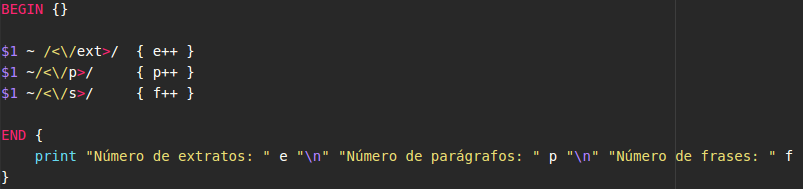
\includegraphics[width=90mm]{alinea1.png} \centering
  \caption{Ficheiro produzido para a 1ª alínea.}
  \label{fig:alinea1}
\end{figure}

\begin{itemize}
	\item \textbf{Extrair a lista das multi-word-expressions e respetivo número de ocorrências}
\end{itemize}
Para esta alínea foi importante a definição do campo \textbf{FS}. Constatamos que cada fator no ficheiro se encontrava separado por \textit{tab}. 
Nesse sentido foi este o valor que \textbf{FS} tomou. De salientar a declaração de uma \textit{string} auxiliar, útil na concatenação das expressões.
Uma vez mais fizemos uso das tag que o documento fornecido apresentava. Sempre que a tag \textit{<mwe ...>} aparecia, inicializamos o contador \textit{C} com o valor um e utilizamos a função \textit{next} facultada pelo \textit{Gawk}. Isto deve-se ao facto de o texto que necessitávamos de retirar não se encontrar nessa linha mas sim na seguinte. Caso o contador apresentasse o valor 1 e caso ainda nos encontrássemos dentro da tag \textit{<mwe ...>} (esta ainda não fechou), recolhíamos o \$1 (primeiro campo que resulta da divisão segundo o FS), incrementávamos o contador e passamos para a linha seguinte. De referir que o contador serve apenas de controlo para o espaço produzido entre as palavras no output. Efetivamente, este não deveria aparecer no inicio de cada linha que será imprimida. Por fim, quando a tag final desta secção é atingida o contador toma o valor de zero e guardamos a string no array associativo para que seja possível calcular o número de ocorrências. O \textit{END} apenas imprime para um ficheiro, que achamos por bem criar para facilitar a visualização dos resultados obtidos.  

\begin{figure}[h!]
  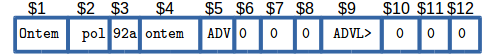
\includegraphics[width=\linewidth]{E1.png}
  \caption{Exemplo da divisão obtida através do FS.}
  \label{fig:example1}
\end{figure}


\begin{figure}[h!]
  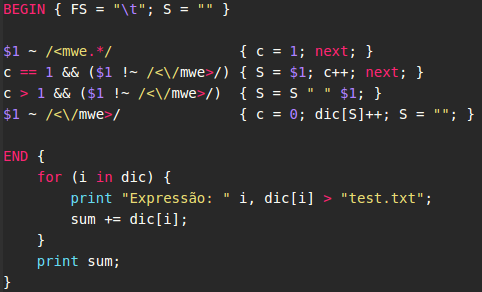
\includegraphics[width=90mm]{alinea2.png} \centering
  \caption{Ficheiro produzido para a 2ª alínea.}
  \label{fig:alinea2}
\end{figure}

\begin{itemize}
	\item \textbf{Calcule a lista dos verbos PT: (Lema, para palavras com pos=V) e respetivo número de ocorrências}
\end{itemize}
Mais uma vez definimos o \textbf{FS} como \textit{"\textbackslash t"} por uma questão de conveniência. Segundo o exemplo, o campo \$5 é onde se apresenta o \textit{part of speech} referido no enunciado(por exemplo o \textit{V}). Novamente, decidimos usar um array associativo, uma vez que este tipo de estrutura permite guardar e contar o número de ocorrências dos resultados mais facilmente. Por fim, apenas imprimimos os valores obtidos.

\begin{figure}[h!]
  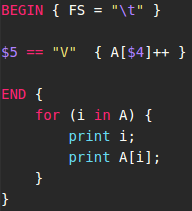
\includegraphics[width=50mm]{alinea3.png} \centering
  \caption{Ficheiro produzido para a 3ª alínea.}
  \label{fig:alinea3}
\end{figure}

\newpage

\begin{itemize}
	\item \textbf{Determinar  o  dicionário  implícito  no  corpora  –  calcule  a  lista  das  palavras  associando-lhes  os  possíveis(lema, pos)} 
\end{itemize}
Na resolução desta alínea é importante destacar o uso de arrays associativos multi-nível. Novamente aproveitamos as tags existentes nos ficheiros fornecidos.


\begin{figure}[h!]
  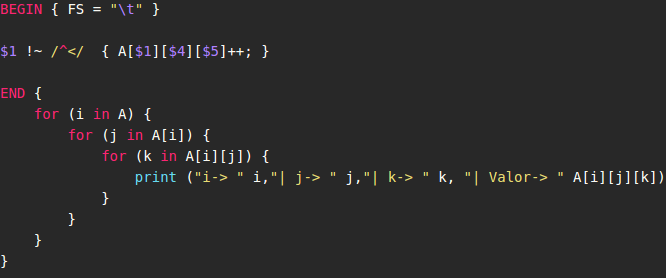
\includegraphics[width=150mm]{alinea4.png} \centering
  \caption{Ficheiro produzido para a 4ª alínea.}
  \label{fig:alinea4}
\end{figure}

\begin{figure}[h!]
  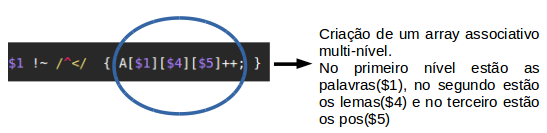
\includegraphics[width=150mm]{ArrayAssociativo.png} \centering
  \caption{Exemplo para a 4ª alínea.}
  \label{fig:alinea4}
\end{figure}





\subsection{Funcionalidades extras}
Uma vez que era encorajado o esforço extra decidimos construir ficheiros \textit{Gawk} para dar resposta a alíneas que não eram abrangidas pelo enunciado. 
As nossas implementações basearam-se na construção de HTML que permitiam uma melhor organização dos dados recolhidos.



 \begin{itemize}
	\item \textbf{Restabelecimento do texto contido nos documentos} 
\end{itemize}
Consideramos que seria útil construir um texto `corrido' com os documentos que nos eram fornecidos. De facto, a forma como texto é apresentado não é, de todo, a mais benéfica para uma leitura eficiente. Assim, recorrendo ao HTML, construimos um índice com o número de extrato correspondente, em que em cada hiperligação se encontra o texto pretendido. É importante realçar o uso das funções \textit{split} e \textit{gsub} neste ficheiro. A primeira foi útil para dividir por espaços toda a tag recolhida. 
Efetivamente, foi necessário usar este processo para obter o número de cada extrato. Neste sentido, para obtermos o número de extrato que estava a ser tratado apenas teríamos de aceder ao segundo campo do array utilizado no \textit{split}.
A função \textit{gsub}, por sua vez, foi utilizada para eliminar o `n=' que se encontrava neste (ver figura 7).    


\begin{figure}[h!]
  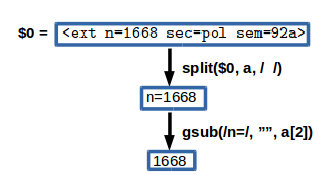
\includegraphics[width=60mm]{Exemplo4.png} \centering
  \caption{Exemplificação da utilização de \textit{split} e \textit{gsub}.}
  \label{fig:Exemplo 4}
\end{figure}


\begin{figure}[h!]
  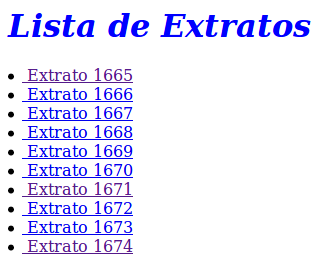
\includegraphics[width=50mm]{htmlExample.png} \centering
  \caption{Novo ficheiro produzido para a 4ª alinea.}
  \label{fig:htmlExample}
\end{figure}

\begin{figure}[h!]
  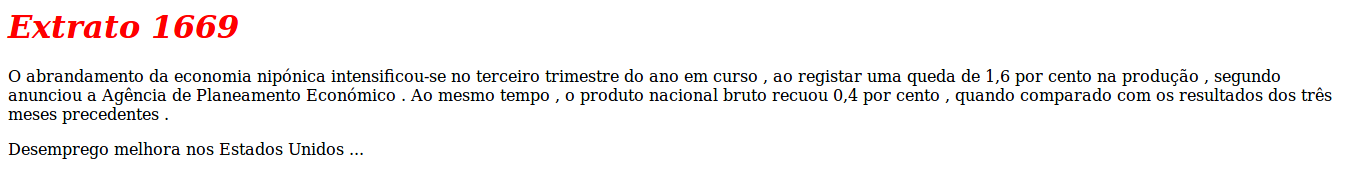
\includegraphics[width=150mm]{htmlExample2.png} \centering
  \caption{Exemplo do resultado obtido.}
  \label{fig:htmlExample2}
\end{figure}

\newpage

 \begin{itemize}
	\item \textbf{Alteração da alínea 4 com a construção de uma tabela} 
\end{itemize}
Consideramos que a criação de um dicionário poderia ser feita de um modo mais prático. Deste modo, facilitamos a visualização dos termos contidos neste com a criação de uma tabela também em HTML.

\begin{verbatim} 
BEGIN {
  FS = "\t"
  s = ""
  print "<html><head><style>\n" > "tabelaDic.html"
  print "table { border-collapse: collapse; width 100%; }\n" > "tabelaDic.html"
  print "th, td { text-align: left; padding: 8px; }\n" > "tabelaDic.html"
  print "tr:nth-child(even){ background-color: #f2f2f2 }\n" > "tabelaDic.html"
  print "th { background-color: #3A80F2; color: white; }\n" > "tabelaDic.html"
  print "</style><meta charset='UTF-8'> </head><body>\n" > "tabelaDic.html"
}
\end{verbatim}

No exemplo acima apresentado, podemos ver o separador de campo como sendo o \textit{tab}. Assim, criamos os ficheiros imprimindo as premissas HTML para estes usando redirecionamento.

\begin{figure}[h!]
  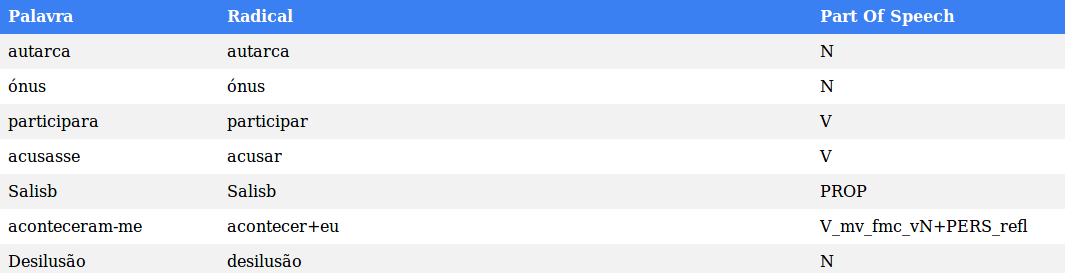
\includegraphics[width=170mm]{exemploTabela.png} \centering
  \caption{Exemplo do resultado obtido.}
  \label{fig:exemploTabela}
\end{figure}

\subsection{Considerações importantes e resultados obtidos}
No decorrer do trabalho não alteramos o campo \textbf{RS} uma vez que o valor \textit{default} deste, enquadrava-se nos objetivos pretendidos. De facto, a escolha apropriada de um \textbf{FS} e um \textbf{RS} facilita bastante o projeto em causa. Por questões de simplificação do relatório, os resultados apresentados dizem respeito ao ficheiro \textit{micro-Cetempublico01.txt}. No entanto, é importante referir que para ficheiros maiores os resultados obtidos continuam dentro do pretendido.

\begin{figure}[h!]
  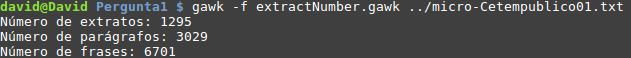
\includegraphics[width=\linewidth]{resultado1.png}
  \caption{Resultados obtidos na alínea 1.}
  \label{fig:r1}
\end{figure}


\begin{figure}[h!]
  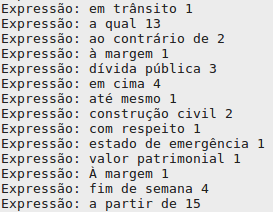
\includegraphics[width=50mm]{resultado2.png} \centering
  \caption{Resultados obtidos na alínea 2.} 
  \label{fig:r2}
\end{figure}


\begin{figure}[h!]
  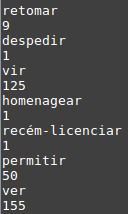
\includegraphics[width=45mm]{resultado3.png} \centering
  \caption{Resultados obtidos na alínea 3.}
  \label{fig:r3}
\end{figure}


\begin{figure}[h!]
  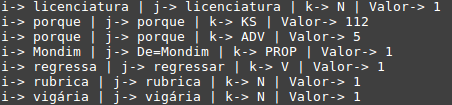
\includegraphics[width=100mm]{resultado4.png} \centering
  \caption{Resultados obtidos na alínea 4.}
  \label{fig:r4}
\end{figure}




\newpage
\mbox{~}
\clearpage
\newpage

\section{Conclusões}
\label{sec:conclusao}
De um modo geral, podemos concluir que os objetivos foram concluídos. De facto, foi possível responder a todas as questões pedidas pelo docente bem como acrescentar outras que consideramos serem úteis. Assim, é importante realçar o interesse revelado por todos os elementos no decorrer da resolução do trabalho.

Os desafios da resolução deste projeto prenderam-se sobretudo com a escolha apropriada do FS. Para além disso, usamos funções(fornecidas pelo Gawk) com as quais não possuíamos contacto prático. No entanto, depois de uma breve pesquisa o restante trabalho surgiu naturalmente. 


Em jeito de conclusão, o presente trabalho serviu para um aprimoramento das nossas aptidões relativamente a uma ferramenta de processamento de texto, Gawk. Efetivamente, foi possível ao grupo concluir o quão poderosas podem ser estas ferramentas. Assim, este trabalho formatou a nossa maneira de pensar aquando da resolução de um problema, tornando-nos mais objetivos e racionais.


\newpage

\section{Bibliografia}
\label{sec:bibliografia}

\begin{itemize}
\item http://www.programacaoprogressiva.net/2012/07/shell-awk-part-i-o-que-e-e-para-que.html acedido no dia 21 pelas 14h;

\item http://natura.di.uminho.pt/~jj/pl-18/ acedido no dia 13 pelas 15h35m.
\end{itemize}

\newpage

\section{Anexos}
\label{sec:anexos}

Código fonte dos exercícios extra:

\small
\begin{verbatim}
BEGIN 
{
FS = "\t";
f = "<li><a href ='%s'> %s </a> </li> \n";
f2 = "<html><body><p> %s ";
print "<h1 style='color:blue;'> <i> Lista de Extratos </i> </h1> \n" > indicegeral.html";
print "<html><head><title>Lista de Extratos</title><meta charset='UTF-8'> </head> \n" > "indicegeral.html";
}

$1 ~ /<ext.*/ 
{
split($0, a, / /);
gsub(/n=/, "", a[2]);
printf (f,"Extrato " a[2] ".html","Extrato " a[2]) > "indicegeral.html";
printf "<html><head><meta charset='UTF-8'> </head> \n"> "Extrato " a[2] .html";
printf ("<h1> <i> <b style = 'color:red'> %s </b> </i> </h1> \n", "Extrato " a[2]) > "Extrato " a[2] ".html";
print "<html><body>" > "Extrato " a[2] ".html"
}

$1 ~ /<p.*/      { print "<p><t>" > "Extrato " a[2] ".html"}

$1 !~ /<.*/      { printf ($1 " ") > "Extrato " a[2] ".html" }

$1 ~ /<\/p>/     { print "</p>" > "Extrato " a[2] ".html" }

$1 ~ /<\/ext>/   { print ("</body></html>") > "Extrato " a[2] ".html" }

END {}

\end{verbatim}

\small
\begin{verbatim}
BEGIN 
{
FS = "\t"
s = ""
print "<html><head><style>\n" > "tabelaDic.html"
print "table { border-collapse: collapse; width 100%; }\n" > "tabelaDic.html"
print "th, td { text-align: left; padding: 8px; }\n" > "tabelaDic.html"
print "tr:nth-child(even){ background-color: #f2f2f2 }\n" > "tabelaDic.html"
print "th { background-color: #3A80F2; color: white; }\n" > "tabelaDic.html"
print "</style><meta charset='UTF-8'> </head><body>\n" > "tabelaDic.html"
}

$1 !~ /^</  { A[$1][$4][$5]++; }

END {
print "<table><tr> <th>Palavra</th> <th>Radical</th>  <th>Part Of Speech</th> </tr>" > "tabelaDic.html"

 for (i in A) {
    for (j in A[i]) {
        for (k in A[i][j]) {
            if (N >= 1) {
               s = s ", " k
            } else {
                 s = k
             }
              N++
         }
    print "<tr><td>" i "</td> <td>" j "</td> <td>" s "</td></tr>" > "tabelaDic.html"
    s = ""
     N = 0
      }
  }

  print "</table></body></html>" > "tabelaDic.html"
}

\end{verbatim}


\end{document}
